\documentclass[a4paper,12pt]{extarticle}
\usepackage[utf8x]{inputenc}
\usepackage[T1,T2A]{fontenc}
\usepackage[russian]{babel}
%% Отступы
\usepackage[left=2cm,right=2cm,top=2cm,bottom=2cm,bindingoffset=0cm]{geometry}

%% Картинки
\usepackage{graphicx} % для картинок
\graphicspath{{fig/}}

%%Точки нумерации заголовков
\usepackage{titlesec}
\titlelabel{\thetitle.\quad}
\usepackage[dotinlabels]{titletoc}

%% Нумерация картинок по секциям
\usepackage{chngcntr}
\counterwithin{figure}{section}
\counterwithin{table}{section}

%% Ставим шрифт Times New Roman
\usepackage{fontspec}
\setmainfont{Times New Roman}

%% Формат картинок
\usepackage{subcaption}
\DeclareCaptionLabelSeparator{custom}{. }
\captionsetup {labelsep=custom}
\addto\captionsrussian{\renewcommand{\figurename}{Рис.}}
\usepackage[belowskip=2pt,aboveskip=2pt]{caption}
\setlength{\intextsep}{2pt plus 1pt minus 1pt}

%% Изменение отступов
\renewcommand{\baselinestretch}{0}
\setlength{\parskip}{0pt}
\setlength{\parindent}{0pt}
\usepackage{titlesec}
\titlespacing*{\section}{0pt}{.5ex plus .5ex minus .5ex}{.5ex plus .5ex}
\titlespacing*{\subsection}{0pt}{.5ex plus .5ex minus .5ex}{.5ex plus .5ex}

%% Изменение оглавления
\usepackage{titletoc}
\titlecontents{section}[0.0cm]{}
{\thecontentslabel\enspace}{}
{{\titlerule*[1pc]{.}\contentspage}}
\titlecontents{subsection}[.4cm]{}
{\thecontentslabel\enspace}{}
{{\titlerule*[1pc]{.}\contentspage}}
\usepackage[unicode]{hyperref}

%% Выравнивание без переносов
\usepackage[none]{hyphenat}
\sloppy

%% Настройка нумерации
\usepackage{fancyhdr}
\pagestyle{fancy}
\fancyhf{}
\fancyfoot[R]{\thepage}
\renewcommand{\headrulewidth}{0pt}
\renewcommand{\footrulewidth}{0pt}
\pagenumbering{arabic}

%% Листинги
\usepackage{listings}
\usepackage{xcolor}

\definecolor{codegreen}{rgb}{0,0.6,0}
\definecolor{codegray}{rgb}{0.5,0.5,0.5}
\definecolor{codeblue}{rgb}{0.58,0,0.82}
\definecolor{backcolour}{rgb}{0.95,0.95,0.92}
\lstset{
    backgroundcolor=\color{backcolour},   
    commentstyle=\color{codegreen},
    keywordstyle=\color{blue},
    numberstyle=\tiny\color{codegray},
    stringstyle=\color{codeblue},
    basicstyle=\ttfamily\footnotesize,
    breakatwhitespace=false,         
    breaklines=true,                 
    captionpos=b,                    
    keepspaces=true,                 
    numbers=left,                    
    numbersep=5pt,                  
    showspaces=false,                
    showstringspaces=false,
    showtabs=false,                  
    tabsize=2
}
\begin{document}

\begin{titlepage}	% начало титульной страницы

	\begin{center}		% выравнивание по центру

		\large Санкт-Петербургский политехнический университет Петра Великого\\[.4cm]
		\large Институт компьютерных наук и кибербезопастности \\[.4cm]
		\large Высшая школа компьютерных технологий и информационных систем\\[6.5cm]
		% название института, затем отступ 6см
		
		\Large \textbf{Отчёт по лабораторной работе №12}\\[0.3cm]
		\large Дисциплина: Телекоммуникационные технологии.\\[5.5cm]

	\end{center}

	\large Выполнил студент гр. 5130901/10101\hfill \underline{\hphantom{(12подпись12)}} \hfill Д.Л. Симоновский\\[.1cm]
	\large \hphantom{Выполнил студент гр. 5130901/10101}\hfill (подпись) \hfill \hphantom{Д.Л. Симоновский}\\[2cm]

	\large Руководитель \hphantom{дент гр. 513090}\hfill \underline{\hphantom{(12подпись12)}} \hfill Н.В. Богач\\[.1cm]
	\large \hphantom{Выполнил студент гр. 5130901/10101}\hfill (подпись) \hfill \hphantom{Д.Л. Симоновский}\\[2cm]

	\hfill\large \today

	\vfill % заполнить всё доступное ниже пространство

	\begin{center}
	\large Санкт-Петербург\\
	\large \the\year % вывести дату
	\end{center} % закончить выравнивание по центру

\end{titlepage} % конец титульной страницы

\vfill % заполнить всё доступное ниже пространство


\renewcommand\contentsname{\centerline{Содержание}}
\tableofcontents
\newpage 

\section{Задача.}\label{sec:s1}
Исследовать применение фильтра низких частот в среде GNU Radio с 
целью понимания его функционала и эффективности в обработке сигналов. 
Основной задачей является изучение способов настройки параметров фильтра 
низких частот для подавления высокочастотных помех и анализ его влияния на 
исходный сигнал. Дополнительной целью является оценка производительности 
фильтра низких частот при различных условиях работы, таких как изменение 
частоты среза и ширины перехода. Полученные результаты помогут глубже понять 
принципы работы фильтров низких частот и их применимость в практических задачах 
обработки сигналов.
\section{Ход работы.}
Начнем исследование с применения фильтра низких частот на косинусоидальный сигнал с частотой 32 кГц.
Для этого соберем следующую схему:\\
\begin{figure}[H]
    \centering
    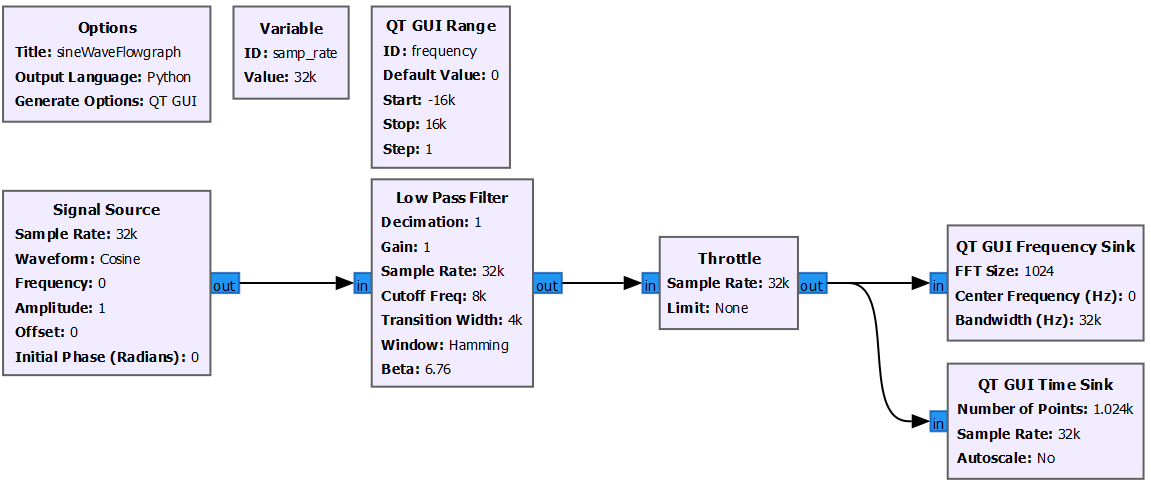
\includegraphics[width=.7\textwidth]{cos_schem}
    \caption{Исследуемая схема.} %% подпись к рисунку
    \label{fig:cos_schem} %% метка рисунка для ссылки на него
\end{figure}
На этой схеме используются следующие блоки:
\begin{itemize}[nolistsep]
    \item \textbf{Varible} - используется для хранения переменной \textit{samp\_rate,} 
    от которой будут отсчитываться остальные частоты в проекте.
    \item \textbf{QT GUI Range} - используется для изменения значения частоты сигнала
    в процессе моделирования.
    \item \textbf{Signal Source} - генератор косинусоидальный сигнала с частотой, подаваемой
    с QT GUI Range и амплитудой 1.
    \item \textbf{Low Pass Filter} - исследуемый фильтр низких частот, он имеет несколько параметров, 
    которые будут рассмотрены позднее. 
    \item \textbf{Throttle} - предназначенный для ограничения скорости передачи сэмплов в цифровой 
    обработке сигналов. Проще говоря ограничитель скорости передачи данных. 
    \item \textbf{QT GUI Frequency Sink} - это графический приемник, основанный на библиотеке QT, 
    предназначенный для отображения нескольких сигналов в частотной области. 
    \item \textbf{QT GUI Time Sink} - это графический приемник, основанный на библиотеке QT, 
    предназначенный для отображения нескольких сигналов во временной области. 
\end{itemize}
Перейдем к рассмотрению настроек \textbf{Low Pass Filter}:\\
\begin{figure}[H]
    \centering
    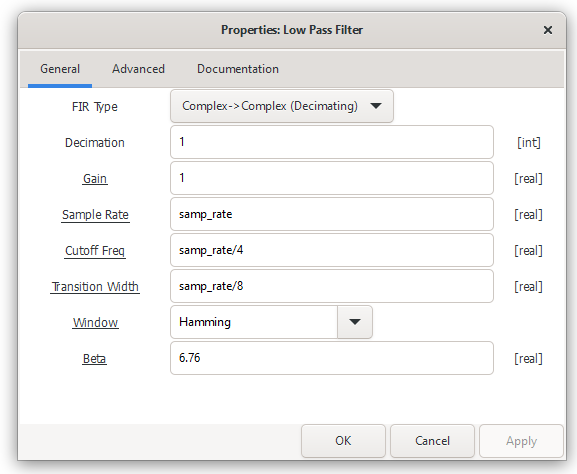
\includegraphics[width=.5\textwidth]{settings_filter}
    \caption{Настройки Low Pass Filter.} %% подпись к рисунку
    \label{fig:settings_filter} %% метка рисунка для ссылки на него
\end{figure}
Рассмотрим подробнее каждый из параметров:
\begin{itemize}[nolistsep]
    \item \textbf{FIR Type} - определяет тип FIR фильтра, то есть указывает, работает ли 
    фильтр с вещественными или комплексными входными/выходными данными.
    \item \textbf{Decimation} - определяет коэффициент децимации фильтра, который указывает, 
    на сколько раз уменьшается частота дискретизации сигнала после применения фильтра.
    \item \textbf{Gain} - масштабирующий коэффициент, применяемый к выходу фильтра, 
    для регулировки амплитуды сигнала.
    \item \textbf{Sample Rate} - частота дискретизации входного сигнала, указывает, с 
    какой частотой входные сигналы отсчитываются во времени. 
    \item \textbf{Cutoff Freq} - частота среза фильтра, то есть частота, на 
    которой фильтр начинает подавлять высокочастотные составляющие входного сигнала.
    \item \textbf{Transition Width} - ширина переходной зоны между полосой подавления 
    и полосой пропускания в фильтре. Этот параметр указывает, насколько широкой 
    должна быть зона плавного перехода между частотами, на которых фильтр полностью 
    подавляет или пропускает сигнал.. 
    \item \textbf{Window} - тип окна, используемого при генерации коэффициентов фильтра. 
    Различные типы окон имеют разные свойства и влияют на характеристики фильтра, такие 
    как разрешение в частотной области и уровень подавления сигнала.
    \item \textbf{Beta} - параметр, который применяется только к окну Кайзера. 
    Этот параметр контролирует форму окна Кайзера и влияет на его способность 
    сглаживания переходной зоны и подавления побочных лепестков.
\end{itemize}
Выполним компиляцию заданной схемы и посмотрим на результат:
\begin{figure}[H]
    \centering
    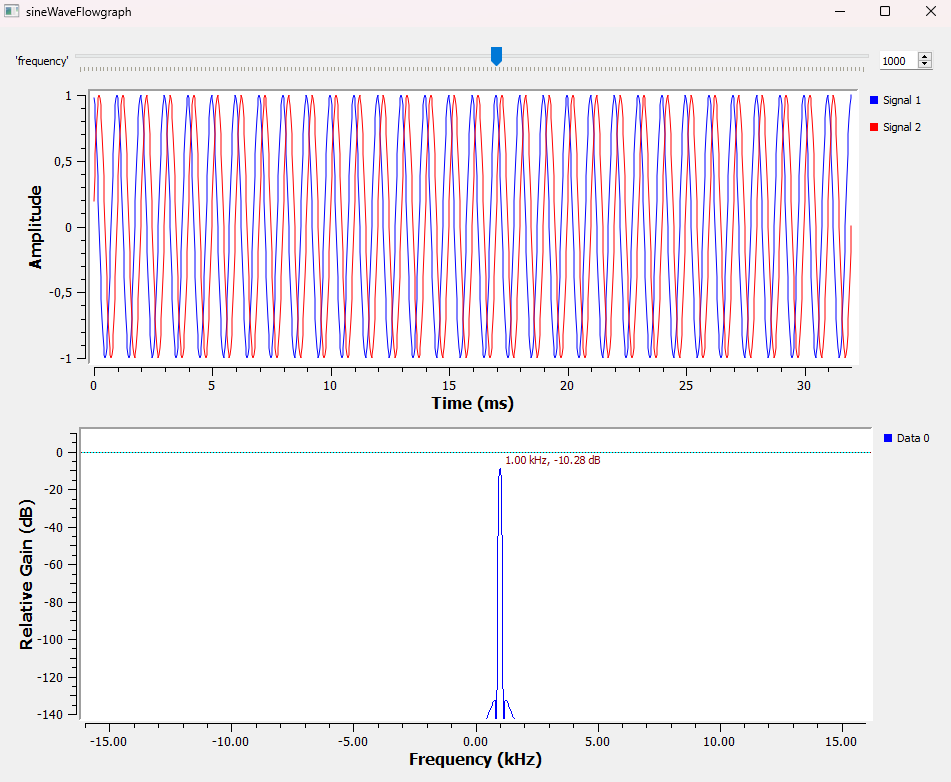
\includegraphics[width=.5\textwidth]{wave_freq_1000}
    \caption{Настройки Low Pass Filter.} %% подпись к рисунку
    \label{fig:wave_freq_1000} %% метка рисунка для ссылки на него
\end{figure}
Как видно на Рис. \ref{fig:wave_freq_1000} мы получили самую обычный косинусоидальный сигнал 
с частотой 1000 и амплитудой 1.\\
Добавим ещё один QT GUI Time Sink на вход сигнала, чтоб отслеживать изменения после фильтра:
\begin{figure}[H]
    \centering
    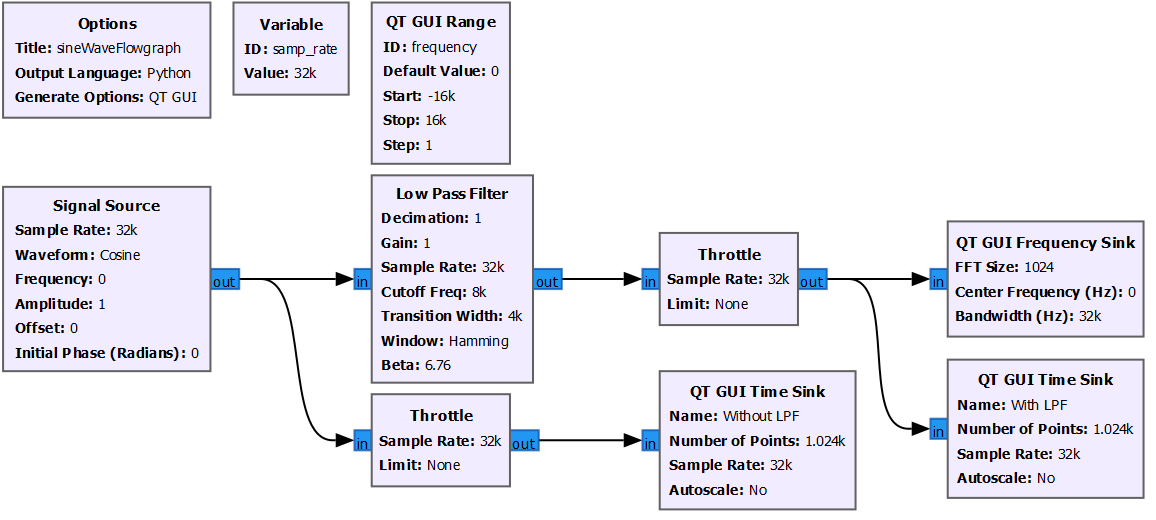
\includegraphics[width=.7\textwidth]{update_schem}
    \caption{Обновленная схема.} %% подпись к рисунку
    \label{fig:update_schem} %% метка рисунка для ссылки на него
\end{figure}
В теории этот Low Pass Filter должен работать следующим образом:
\begin{itemize}[nolistsep]
    \item В промежутке от 0 до 4 кГц не должно быть никаких изменений.
    \item В промежутке от 4 кГц до 8 кГц амплитуда должна упасть в 2 раза.
    \item В промежутке от 8 кГц до 12 кГц амплитуда должна упасть практически до 0.
\end{itemize}
Проверим это, сделав несколько замеров:
\begin{figure}[H]
    \centering
    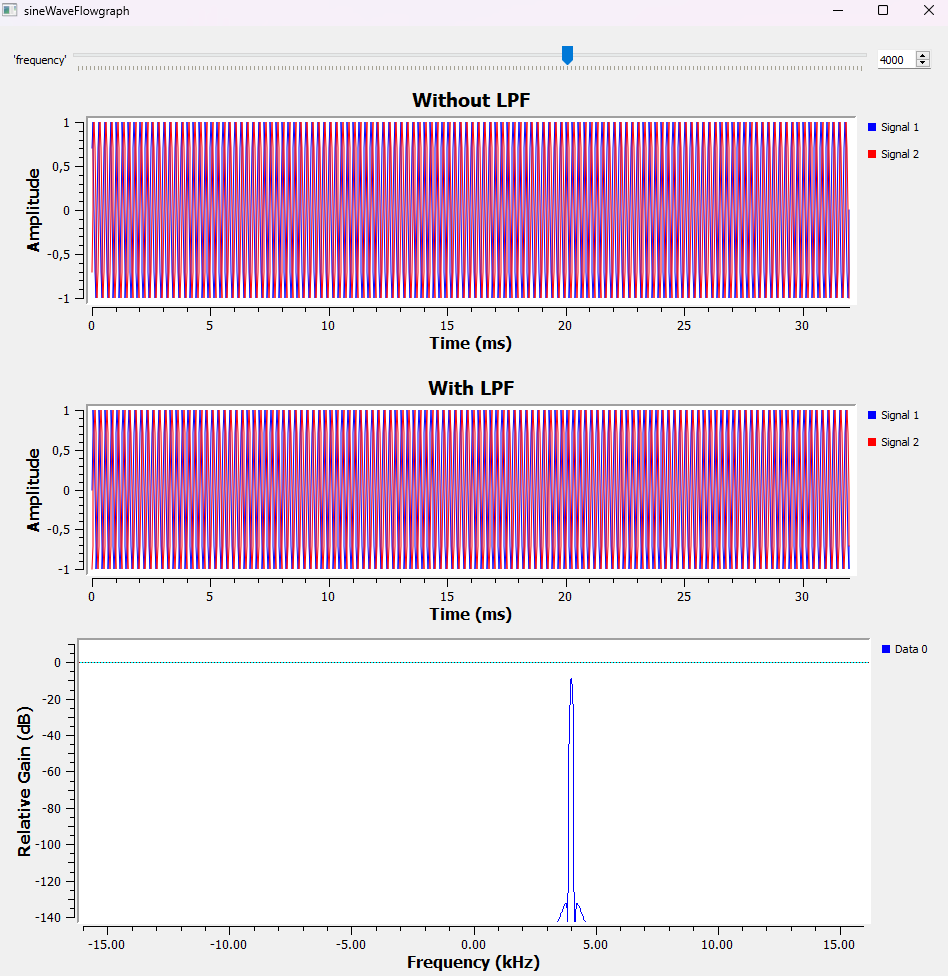
\includegraphics[width=.5\textwidth]{wave_freq_4000.png}
    \caption{Frequency = 4000 Гц.} %% подпись к рисунку
    \label{fig:wave_freq_4000} %% метка рисунка для ссылки на него
\end{figure}
\begin{figure}[H]
    \centering
    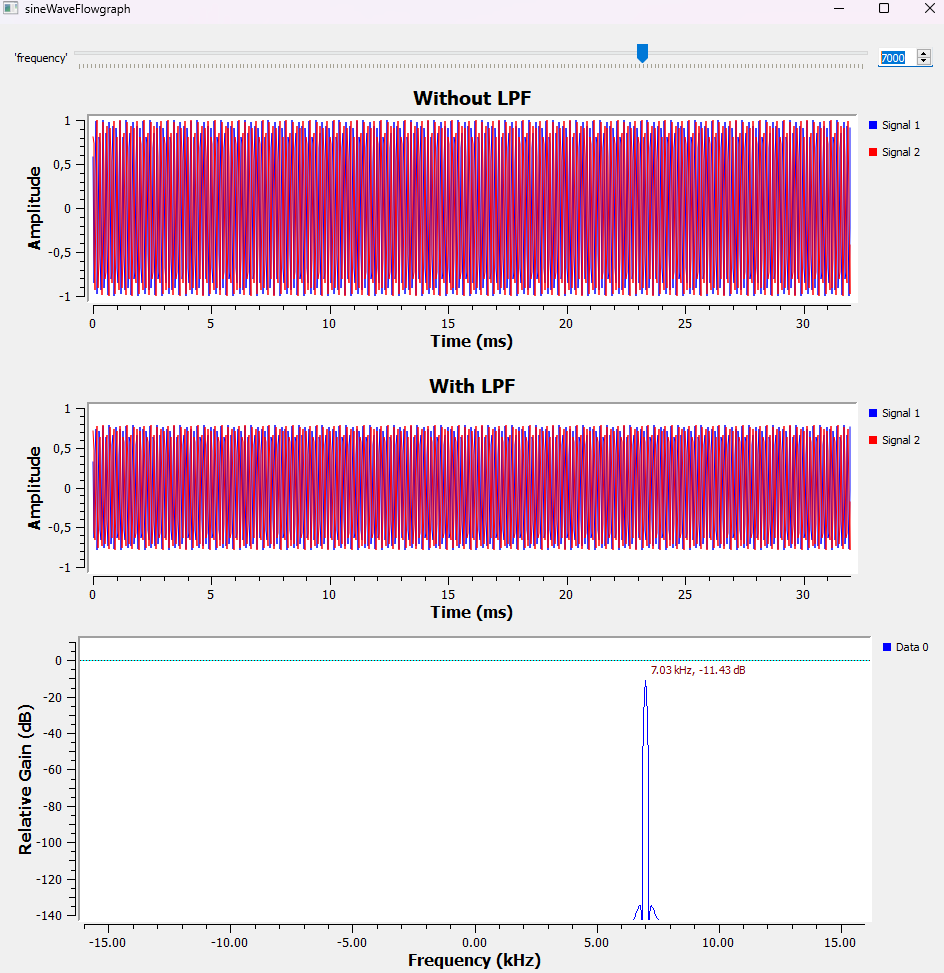
\includegraphics[width=.5\textwidth]{wave_freq_7000.png}
    \caption{Frequency = 7000 Гц.} %% подпись к рисунку
    \label{fig:wave_freq_7000} %% метка рисунка для ссылки на него
\end{figure}
Как можно заметить по рисункам выше, действительно, начиная с 4 кГц амплитуда сигнала
начинает спадать. Рассмотрим сигнал на 8 кГц:
\begin{figure}[H]
    \centering
    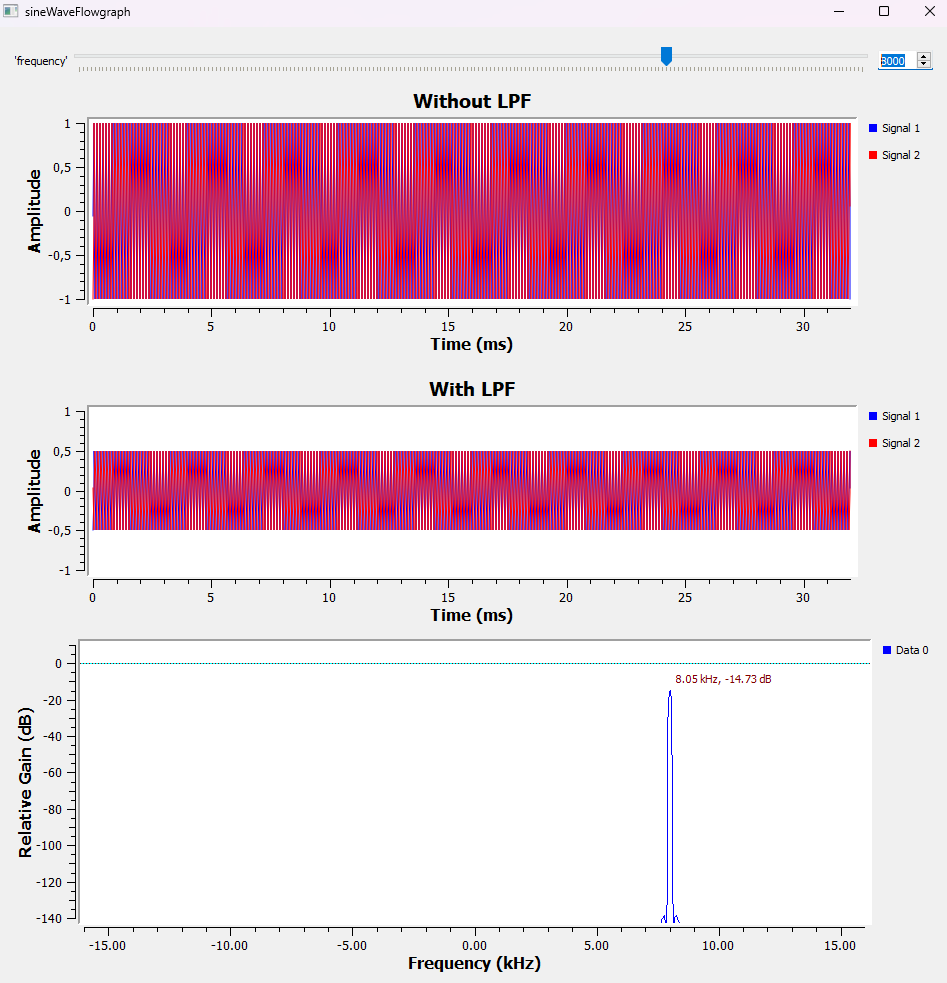
\includegraphics[width=.5\textwidth]{wave_freq_8000.png}
    \caption{Frequency = 8000 Гц.} %% подпись к рисунку
    \label{fig:wave_freq_8000} %% метка рисунка для ссылки на него
\end{figure}
Видим, что как и было предсказано при частоте, равной Cutoff Freq, амплитуда сигнала
уменьшилась вдвое. Посмотрим что будет при дальнейшем увеличении частоты:
\begin{figure}[H]
    \centering
    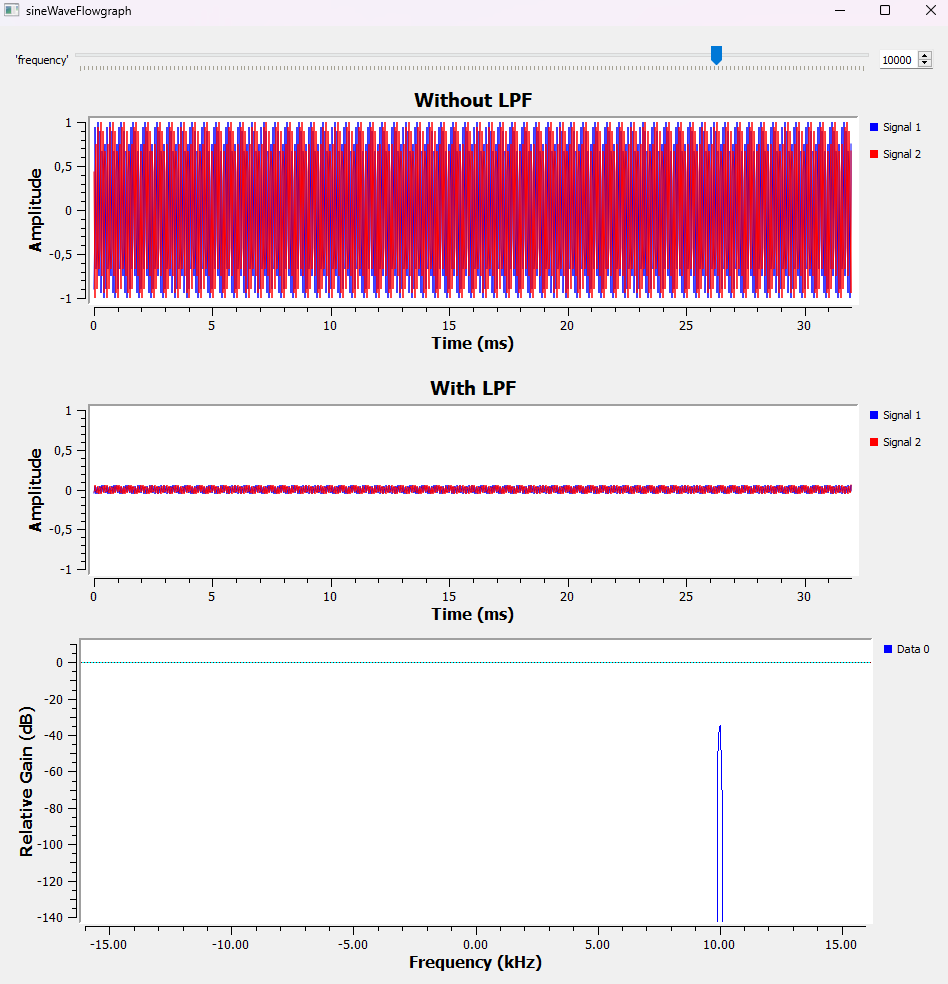
\includegraphics[width=.5\textwidth]{wave_freq_10000.png}
    \caption{Frequency = 10000 Гц.} %% подпись к рисунку
    \label{fig:wave_freq_10000} %% метка рисунка для ссылки на него
\end{figure}
\begin{figure}[H]
    \centering
    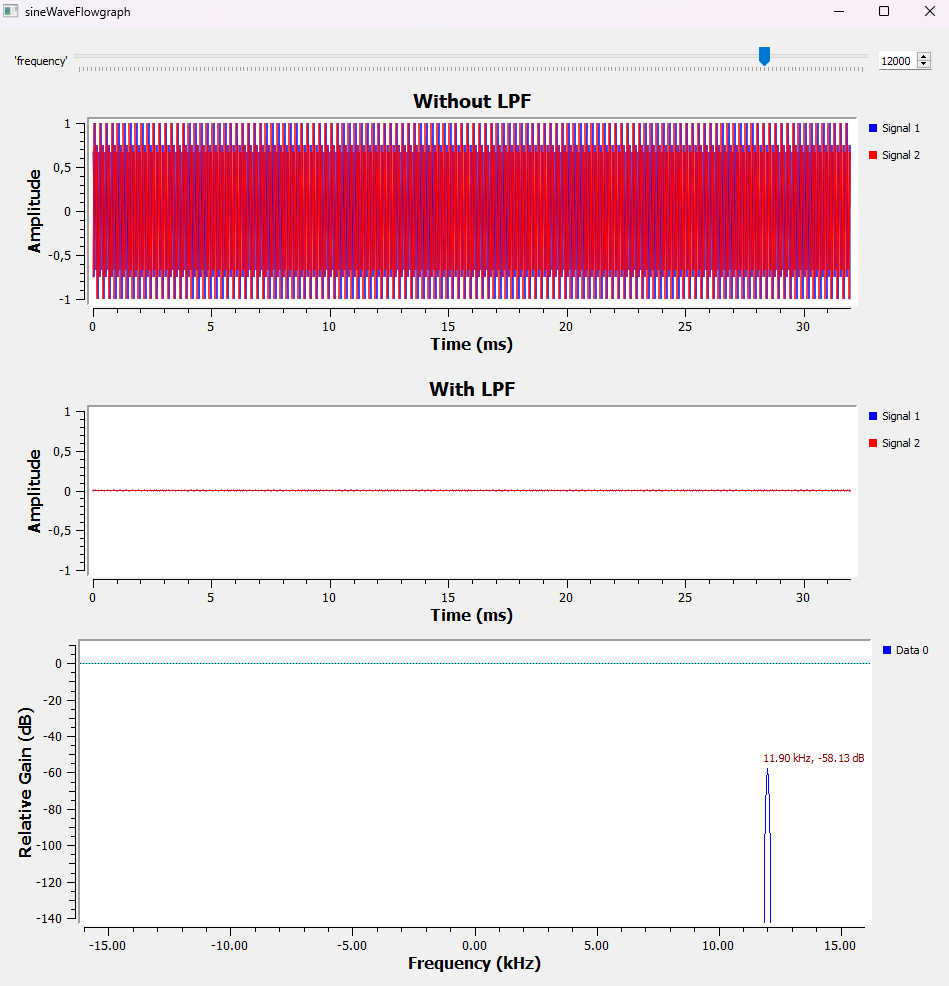
\includegraphics[width=.5\textwidth]{wave_freq_12000.png}
    \caption{Frequency = 12000 Гц.} %% подпись к рисунку
    \label{fig:wave_freq_12000} %% метка рисунка для ссылки на него
\end{figure}
Как видим, при 12 кГц частота уменьшилась во много раз и итоговый сигнал 
практически не различим.\\
Для более наглядной демонстрации, вместо изменения частоты косинусоидального сигнала, 
заменим сигнал на входе на шум:
\begin{figure}[H]
    \centering
    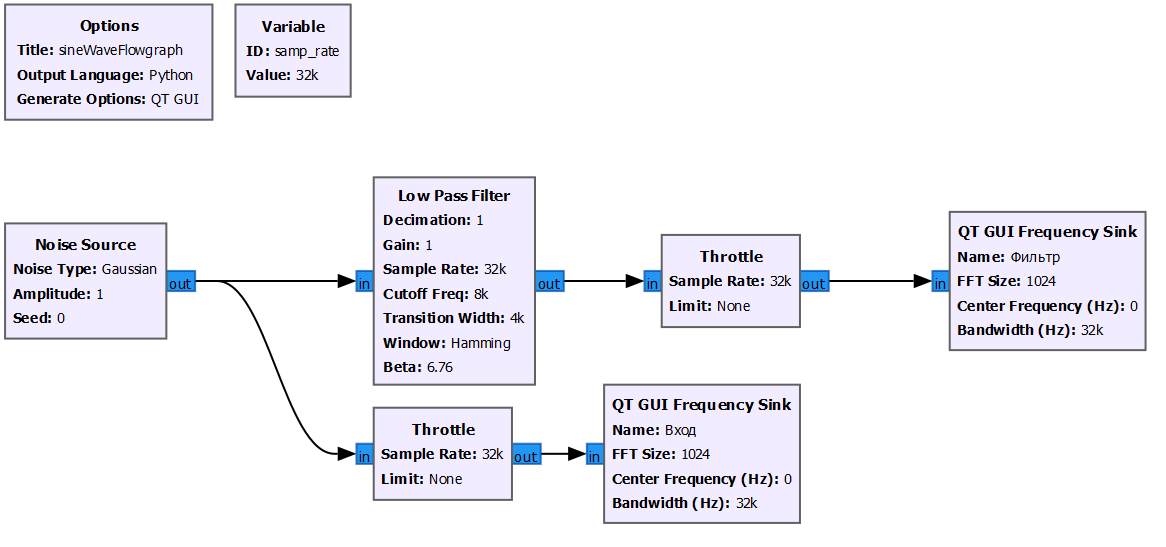
\includegraphics[width=.7\textwidth]{noise_schem.png}
    \caption{Схема на шуме Гаусса.} %% подпись к рисунку
    \label{fig:noise_schem} %% метка рисунка для ссылки на него
\end{figure}
Т.к. шум Гаусса - белый, ожидается одинаковое значение на всех частотах, что мы увидим 
на QT GUI Frequency Sink. Однако после фильтра низких частот, все частоты выше 12 кГц 
должны исчезнуть полностью, а с 8 кГц по 12 кГц значительно уменьшиться:
\begin{figure}[H]
    \centering
    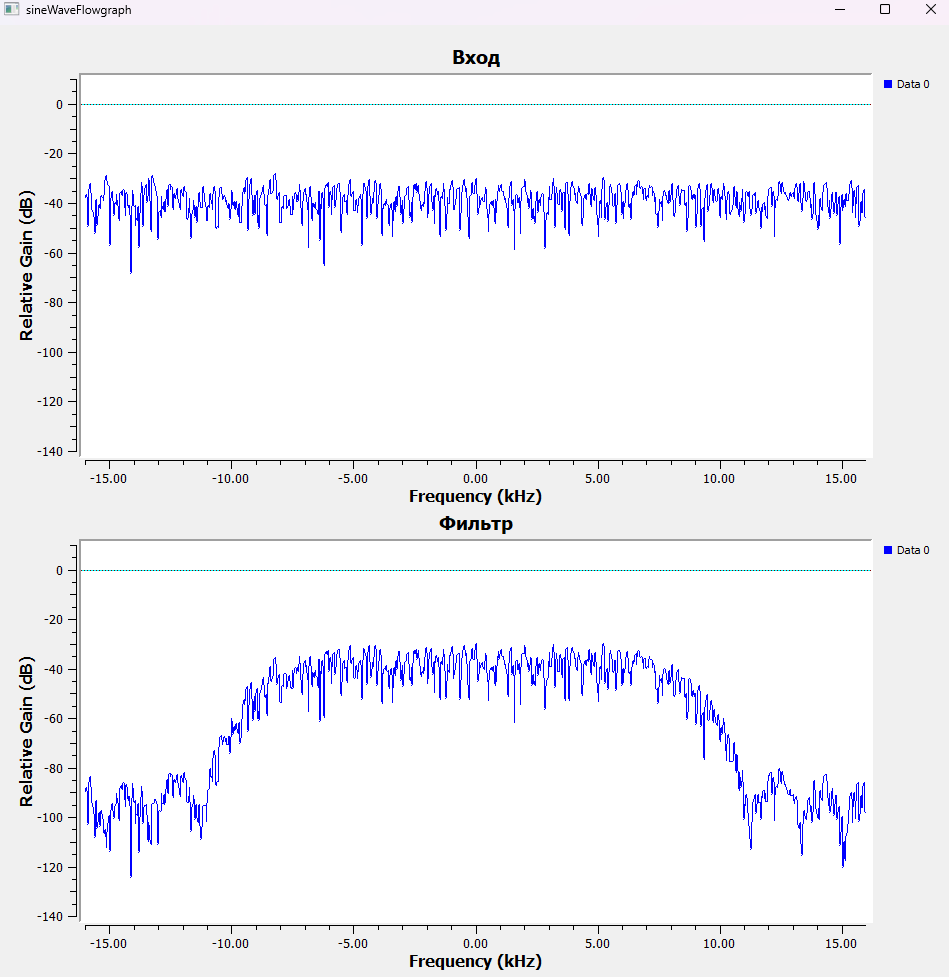
\includegraphics[width=.5\textwidth]{filtered_noise.png}
    \caption{Графики схемы на шуме Гаусса.} %% подпись к рисунку
    \label{fig:filtered_noise} %% метка рисунка для ссылки на него
\end{figure}
И действительно, именно этот эффект мы и наблюдаем выше.
\section{Вывод.}
В результате работы было показано, что фильтр низких частот эффективно 
подавляет высокочастотные помехи, а также способен корректно обрабатывать 
сигналы с различными частотами. Наблюдаемые изменения амплитуды сигнала после 
применения фильтра соответствовали ожиданиям и подтверждали правильность его настройки.\\
Также было продемонстрировано, что фильтр низких частот успешно применяется не 
только к косинусоидальным сигналам, но и к шуму, что подтверждает его 
универсальность и применимость в различных сценариях обработки сигналов.\\
Таким образом, можно сделать вывод, что исследование позволило глубже 
понять принципы работы фильтров низких частот и их применимость в 
практических задачах обработки сигналов в среде GNU Radio.\\
\end{document}